\documentclass[11pt,a4paper]{article}

\usepackage[margin=1in]{geometry}
\usepackage{graphicx}
\usepackage{booktabs}
\usepackage{multirow}
\usepackage{array}
\usepackage{tabularx}
\usepackage{amsmath,amssymb}
\usepackage{enumitem}
\usepackage{hyperref}
\usepackage{xcolor}
\usepackage{float}

\hypersetup{
	colorlinks=true,
	linkcolor=blue,
	citecolor=blue,
	urlcolor=blue
}

\title{GNR 638: Assignment 2 Report\\
\large Pre-trained CNN Representation Transfer and Robustness Analysis}
\author{Avinash Chaudhari, Pranay Marumamula \\ 23b1064, 23b1073}
\date{\today}

\begin{document}
\maketitle

\begin{abstract}
This report presents a comprehensive evaluation of pre-trained convolutional neural network (CNN) representations for remote sensing image classification. We analyze three backbones (ResNet50, EfficientNet-B0, ConvNeXt-Tiny) across linear probe transfer, fine-tuning strategy comparison (linear probe, last-block, selective unfreezing, full fine-tuning), few-shot learning, layer-wise feature probing, and corruption robustness on the Aerial Image Dataset. Results show clear trade-offs: EfficientNet-B0 is most data-efficient in few-shot settings, fine-tuning outcomes are model-dependent (ResNet50: last-block/selective tie; EfficientNet-B0: full fine-tuning best; ConvNeXt-Tiny: selective best), ConvNeXt-Tiny provides the strongest robustness under corruption and the best probe accuracy at middle depth, and ResNet50 achieves very high linear-probe transfer performance on the available logged run. Overall, the experiments highlight that optimal representation quality depends on the target criterion (data efficiency, adaptation budget, separability across depth, or robustness under distribution shift).
\end{abstract}

\tableofcontents
\newpage

\section{Introduction}
\subsection{Background}
Remote sensing scene classification is a transfer-learning-heavy problem because labeled aerial datasets are much smaller than large-scale natural image corpora such as ImageNet. In this assignment, we study how effectively ImageNet pre-trained CNN backbones transfer to AID (30-class aerial scene classification) under practical constraints such as limited supervision and distribution shift. The selected backbones represent different design families: residual connections (ResNet50), compound scaling (EfficientNet-B0), and modernized convolutional design (ConvNeXt-Tiny).

To evaluate representation quality beyond a single clean accuracy number, we follow a multi-scenario protocol implemented in our codebase: (i) linear probe transfer with a frozen backbone and trainable final classifier, (ii) fine-tuning strategy comparison (linear probe vs partial/full unfreezing), (iii) few-shot analysis by training on $100\%$, $20\%$, and $5\%$ of training data, (iv) layer-wise probing using linear classifiers on early/middle/final intermediate features, and (v) corruption robustness testing under Gaussian noise, motion blur, and brightness shift. Together, these analyses characterize transferability, adaptation-efficiency trade-offs, data efficiency, feature hierarchy, and robustness sensitivity of pre-trained representations.

\subsection{Objectives}
The main objectives of this report are:
\begin{itemize}
	\item Compare the transfer performance of ResNet50, EfficientNet-B0, and ConvNeXt-Tiny on AID using a consistent training and evaluation protocol.
	\item Compare fine-tuning strategies (linear probe, last-block unfreezing, selective unfreezing, and full fine-tuning) under matched optimization settings.
	\item Quantify data efficiency in few-shot regimes ($100\%$, $20\%$, $5\%$ train data) and measure relative performance drop and training-validation gap.
	\item Evaluate linear-probe transferability by freezing the backbone and training only the final linear head.
	\item Analyze semantic abstraction across depth via layer-wise feature probing (early, middle, final layers) using linear classifiers and feature statistics.
	\item Benchmark robustness under controlled corruptions and study architecture-dependent sensitivity under distribution shift.
\end{itemize}

\section{Dataset and Experimental Setup}
\subsection{Dataset}
We use the Aerial Image Dataset (AID) provided in image-folder format (one subfolder per class). In our local setup, the training directory \texttt{train\_data/} contains 30 scene classes and 6993 images in total. The class distribution is imbalanced, with per-class sample count ranging from 154 to 294 images.

The 30 classes are: Airport, BareLand, BaseballField, Beach, Bridge, Center, Church, Commercial, DenseResidential, Desert, Farmland, Forest, Industrial, Meadow, MediumResidential, Mountain, Park, Parking, Playground, Pond, Port, RailwayStation, Resort, River, School, SparseResidential, Square, Stadium, StorageTanks, and Viaduct. The assignment also specifies a fixed hidden test set for grading; therefore, all analysis in this report is based on training/validation protocols implemented in the submitted code.

Across scripts, splits are scenario-specific but seed-controlled:
\begin{itemize}
	\item \textbf{Few-shot scripts:} random $80/20$ train/validation split, then train subset sampling at $100\%$, $20\%$, and $5\%$ of train data.
	\item \textbf{Layer-wise probing scripts:} stratified $80/20$ split using \texttt{train\_test\_split} with \texttt{stratify=targets}.
	\item \textbf{Linear-probe transfer scripts:} random $70/30$ train/validation split.
\end{itemize}

Input preprocessing follows ImageNet conventions for compatibility with pre-trained weights. Most models use resize to $224\times224$, tensor conversion, and normalization with mean $[0.485,0.456,0.406]$ and std $[0.229,0.224,0.225]$. Inception-v3 based transfer scripts use $299\times299$. Training transforms in transfer scripts include random horizontal flip.

\subsection{Implementation Details}
All experiments are implemented in PyTorch using \texttt{torchvision} pre-trained backbones. The primary models evaluated in this report are ResNet50, EfficientNet-B0, and ConvNeXt-Tiny, initialized from ImageNet weights and adapted to 30 output classes by replacing the final classifier layer.

Reproducibility controls are explicitly used in code (seed $=42$ for NumPy/PyTorch, and explicit seeded generators in split/checkpoint-evaluation scripts).

The training setup used in code is summarized below:
\begin{itemize}
	\item \textbf{Few-shot analysis:} optimizer Adam, learning rate $10^{-3}$, batch size 32, up to 20 epochs per regime.
	\item \textbf{Linear probe transfer:} frozen backbone (for linear-probe runs), Adam with learning rate $10^{-4}$ over trainable classifier parameters, batch size 32, 30 epochs, \texttt{num\_workers}=2.
	\item \textbf{Layer-wise feature probing:} frozen pre-trained feature extractor, linear probes via logistic regression on extracted features, batch size 64, \texttt{num\_workers}=4, and fixed PCA subset of 30 classes $\times$ 30 samples/class.
	\item \textbf{Device:} scripts use automatic device selection (CUDA if available, else CPU).
\end{itemize}

\section{Linear Probe Transfer}
\subsection{Methodology}
Linear probe transfer evaluates how separable pretrained features are when only a linear classifier is trained on top of them. In the provided scripts under \texttt{linear\_probe\_transfer/}, each model is adapted to 30 AID classes by replacing the final classification layer. The evaluation/plot scripts load saved checkpoints and generate validation diagnostics without any retraining.

For the three models considered in this report (ResNet50, EfficientNet-B0, ConvNeXt-Tiny), the common setup is:
\begin{itemize}
	\item Validation split: $30\%$ (seed 42)
	\item Batch size: 32, \texttt{num\_workers}=2
	\item Input preprocessing: resize to $224\times224$, ImageNet normalization
	\item Diagnostics generated from checkpoints: training-validation accuracy curve, confusion matrix (row-normalized \%), PCA embedding plot, and t-SNE embedding plot
\end{itemize}

The main transfer metric reported is validation accuracy. Class separability and failure patterns are analyzed through confusion matrices and embedding visualizations.

\subsection{Results}
\begin{table}[H]
	\centering
	\caption{Linear probe transfer summary (ResNet50 log + checkpoint visual diagnostics).}
	\begin{tabular}{lcc}
		\toprule
		Model & Best Val Acc (\%) & Final Test/Val Acc (\%) \\
		\midrule
		ResNet50 & 98.28 & 98.28 \\
		EfficientNet-B0 & 87.37 & 87.37 \\
		ConvNeXt-Tiny & 95.28 & 95.28 \\
		\bottomrule
	\end{tabular}
\end{table}

Based on the values summarized in Table 3.1, linear-probe transfer is strongest for ResNet50 ($98.28\%$), followed by ConvNeXt-Tiny ($95.28\%$), and then EfficientNet-B0 ($87.37\%$). For all three models, the reported best and final validation values are identical in the exported artifacts, indicating stable end-of-training performance in these runs.

\subsubsection*{ResNet50 linear-probe plots}
\begin{figure}[H]
	\centering
	
\includegraphics[width=0.75\textwidth]{../linear_probe_transfer/resnet50_linear_probe_transfer/training_validation_acc.png}
	\caption{ResNet50: training vs validation accuracy.}
\end{figure}

\begin{figure}[H]
	\centering
	
\includegraphics[width=0.75\textwidth]{../linear_probe_transfer/resnet50_linear_probe_transfer/confusion_matrix.png}
	\caption{ResNet50: confusion matrix on validation split (\%).}
\end{figure}

\begin{figure}[H]
	\centering
	
\includegraphics[width=0.75\textwidth]{../linear_probe_transfer/resnet50_linear_probe_transfer/embeddings_pca.png}
	\caption{ResNet50: PCA projection of validation embeddings.}
\end{figure}

\begin{figure}[H]
	\centering
	
\includegraphics[width=0.75\textwidth]{../linear_probe_transfer/resnet50_linear_probe_transfer/embeddings_tsne.png}
	\caption{ResNet50: t-SNE projection of validation embeddings.}
\end{figure}

\subsubsection*{EfficientNet-B0 linear-probe plots}
\begin{figure}[H]
	\centering
	
\includegraphics[width=0.75\textwidth]{../linear_probe_transfer/efficientnet_b0_linear_probe_transfer/training_validation_acc.png}
	\caption{EfficientNet-B0: training vs validation accuracy.}
\end{figure}

\begin{figure}[H]
	\centering
	
\includegraphics[width=0.75\textwidth]{../linear_probe_transfer/efficientnet_b0_linear_probe_transfer/confusion_matrix.png}
	\caption{EfficientNet-B0: confusion matrix on validation split (\%).}
\end{figure}

\begin{figure}[H]
	\centering
	
\includegraphics[width=0.75\textwidth]{../linear_probe_transfer/efficientnet_b0_linear_probe_transfer/embeddings_pca.png}
	\caption{EfficientNet-B0: PCA projection of validation embeddings.}
\end{figure}

\begin{figure}[H]
	\centering
	
\includegraphics[width=0.75\textwidth]{../linear_probe_transfer/efficientnet_b0_linear_probe_transfer/embeddings_tsne.png}
	\caption{EfficientNet-B0: t-SNE projection of validation embeddings.}
\end{figure}

\subsubsection*{ConvNeXt-Tiny linear-probe plots}
\begin{figure}[H]
	\centering
	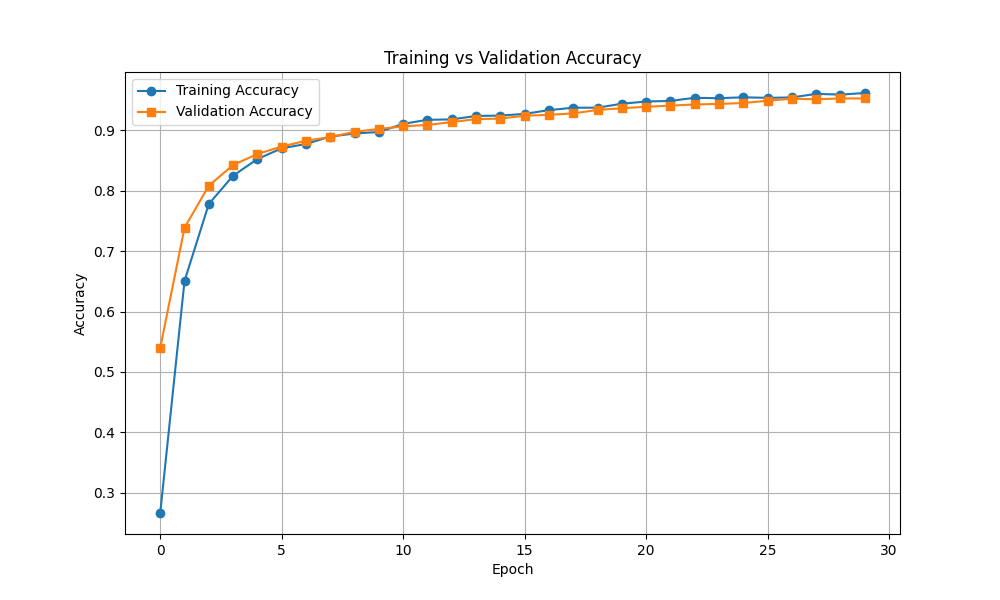
\includegraphics[width=0.75\textwidth]{../linear_probe_transfer/convnext_tiny_linear_probe_transfer/training_validation_acc.png}
	\caption{ConvNeXt-Tiny: training vs validation accuracy.}
\end{figure}

\begin{figure}[H]
	\centering
	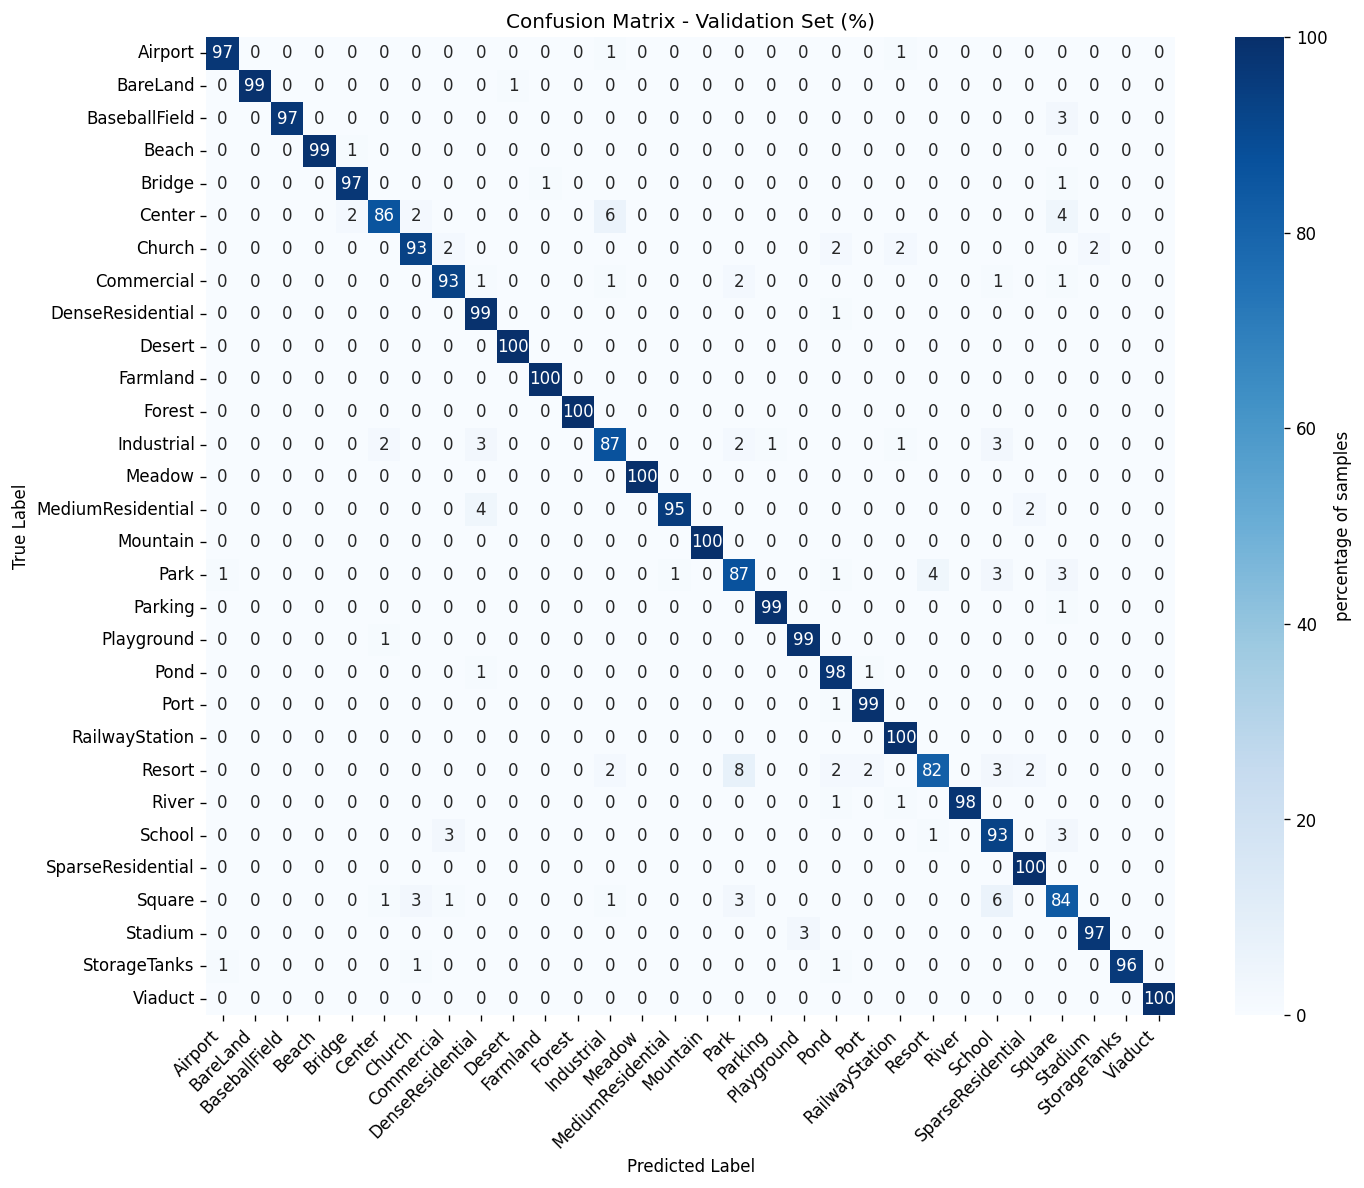
\includegraphics[width=0.75\textwidth]{../linear_probe_transfer/convnext_tiny_linear_probe_transfer/confusion_matrix.png}
	\caption{ConvNeXt-Tiny: confusion matrix on validation split (\%).}
\end{figure}

\begin{figure}[H]
	\centering
	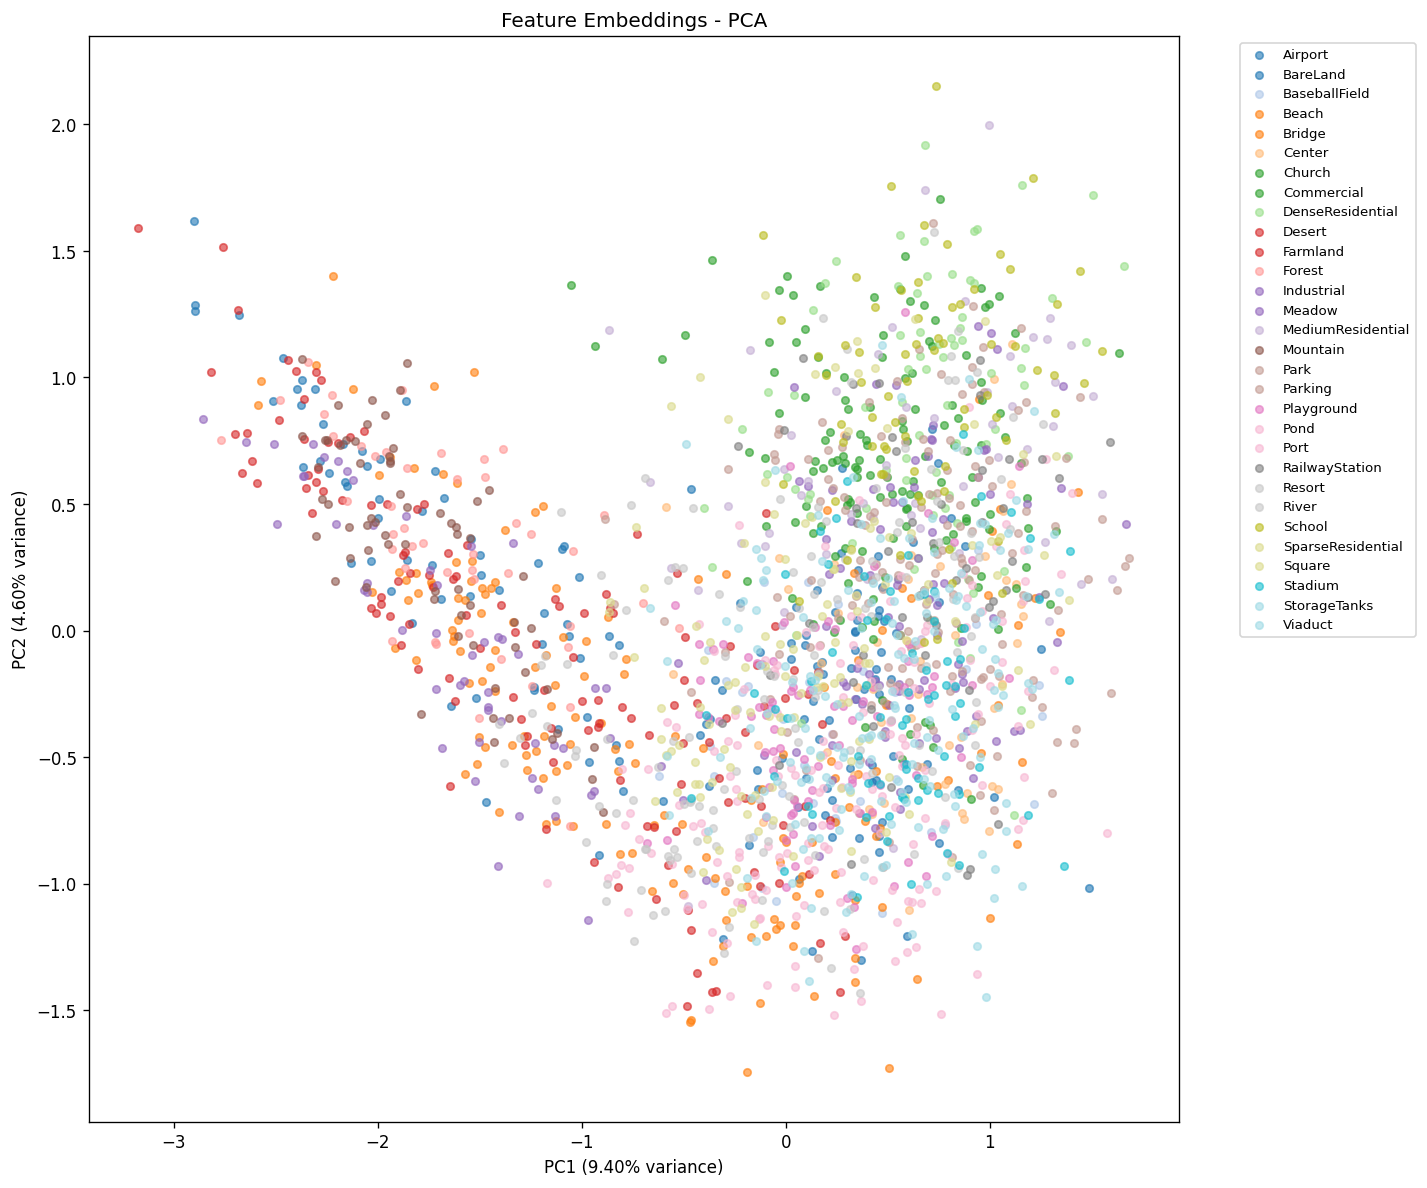
\includegraphics[width=0.75\textwidth]{../linear_probe_transfer/convnext_tiny_linear_probe_transfer/embeddings_pca.png}
	\caption{ConvNeXt-Tiny: PCA projection of validation embeddings.}
\end{figure}

\begin{figure}[H]
	\centering
	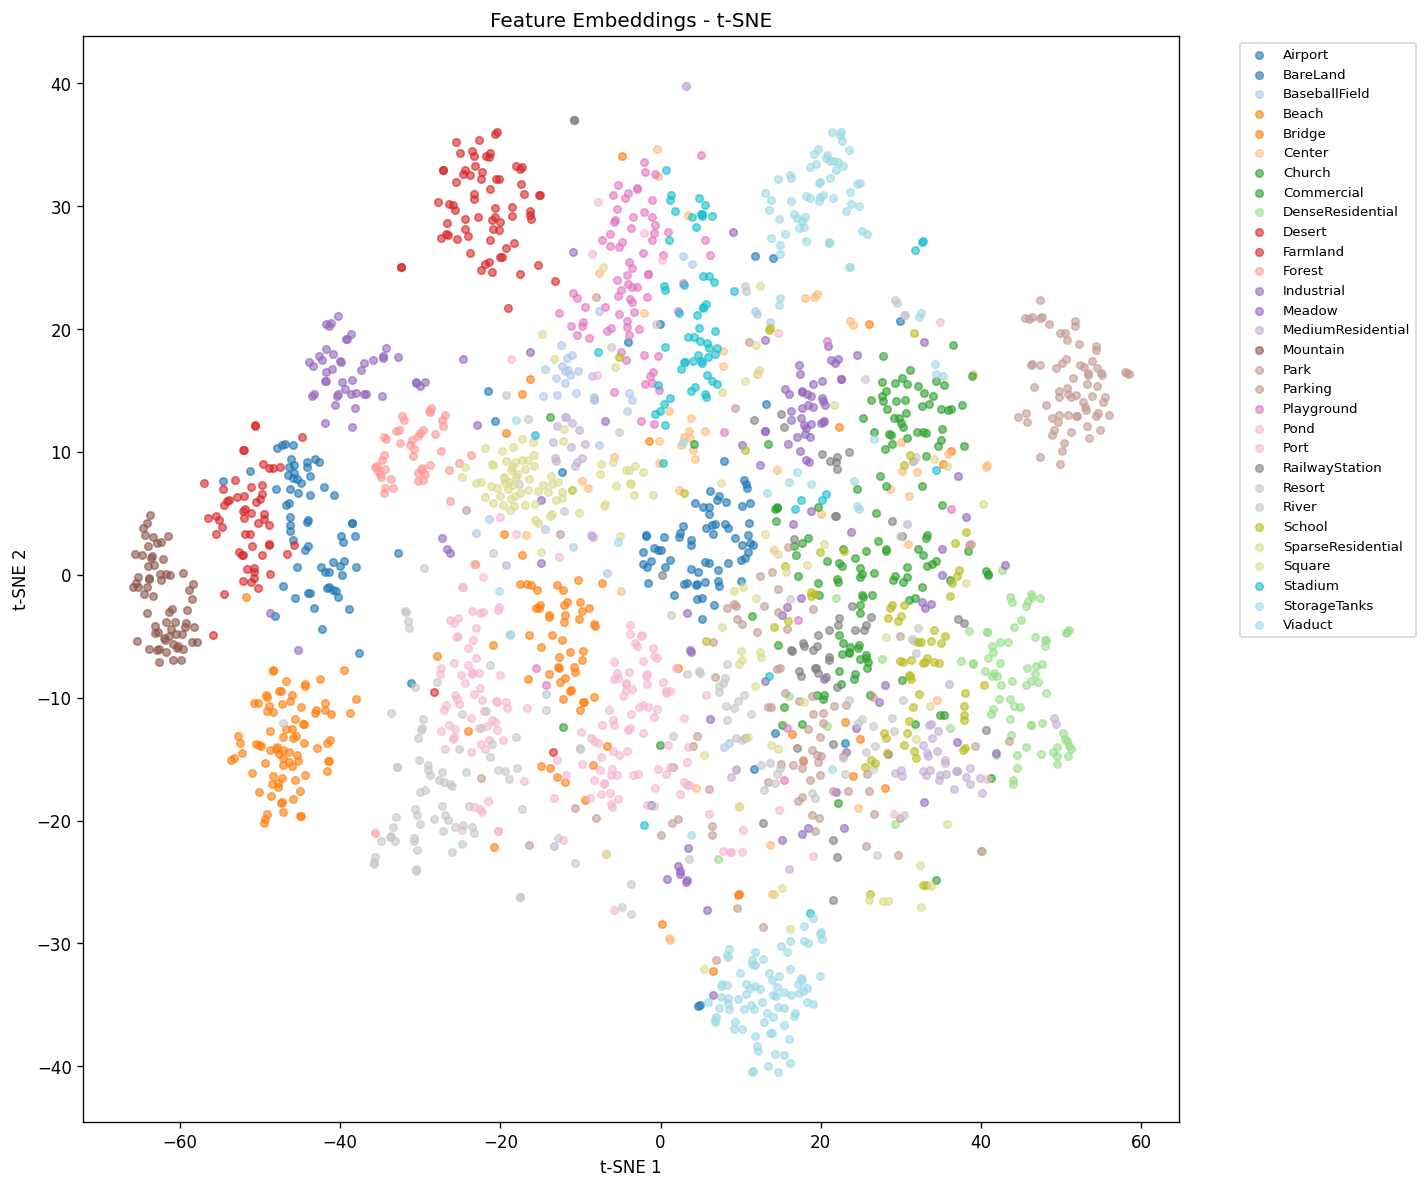
\includegraphics[width=0.75\textwidth]{../linear_probe_transfer/convnext_tiny_linear_probe_transfer/embeddings_tsne.png}
	\caption{ConvNeXt-Tiny: t-SNE projection of validation embeddings.}
\end{figure}

\subsection{Training Dynamics}
Across all three models, training-validation curves show rapid early improvement followed by stabilization, consistent with strong transfer from ImageNet-pretrained features. The final validation accuracy is highest for ResNet50 (98.28\%), followed by ConvNeXt-Tiny (95.28\%), and EfficientNet-B0 (87.37\%).

Confusion matrices indicate that most classes are well recognized, while residual errors are concentrated in visually similar scene categories (for example, dense/medium/sparse residential and some land-cover classes). PCA and t-SNE plots show largely separable class clusters with partial overlap among semantically close classes, which is expected for linear probing on aerial scenes.

\section{Fine-Tuning Strategies}

\subsection{Methodology}
Fine-tuning strategy comparison evaluates how different degrees of backbone parameter unfreezing affect transfer performance, convergence stability, and gradient flow. For each of the three backbones (ResNet50, EfficientNet-B0, ConvNeXt-Tiny), we implement four distinct strategies:

\begin{itemize}
	\item \textbf{Linear probe:} Freeze all backbone parameters; train only the classifier head.
	\item \textbf{Last block fine-tuning:} Freeze early and middle layers; unfreeze the final residual/feature block and classifier.
	\item \textbf{Full fine-tuning:} Unfreeze all backbone parameters and the classifier for end-to-end training.
	\item \textbf{Selective layer unfreezing:} Strategically unfreeze a limited set ($\approx 20\%$ of total backbone parameters) to balance adaptation and stability.
\end{itemize}

All strategies use identical hyperparameters for fair comparison:
\begin{itemize}
	\item Data split: $70/30$ train/validation (seed 42)
	\item Optimizer: Adam with learning rate $10^{-4}$ on trainable parameters only
	\item Batch size: 32, \texttt{num\_workers}=2
	\item Training epochs: 20
	\item Input preprocessing: resize to $224\times224$, ImageNet normalization, random horizontal flip during training
\end{itemize}

\subsubsection*{Selective unfreezing rationale}
For selective unfreezing at approximately $20\%$ budget, layers are chosen based on architectural depth and parameter density:

\begin{itemize}
	\item \textbf{ResNet50 (14.3\% unfrozen):} Last three residual blocks of \texttt{layer3} plus classifier. Rationale: layer3 contains the deepest, task-specific features while avoiding the expensive fully-connected layers.
	\item \textbf{EfficientNet-B0 (20.38\% unfrozen):} Features blocks 4 and 5 (MBConv blocks with high capacity) plus classifier. Rationale: EfficientNet's compound scaling concentrates semantic features in later MBConv stages.
	\item \textbf{ConvNeXt-Tiny (17.28\% unfrozen):} Feature blocks 5 and 6 (including the downsampling stage) plus classifier. Rationale: ConvNeXt's design emphasizes modern convolution blocks in the deeper half; block 6 includes important spatial consolidation.
\end{itemize}

All runs track per-layer gradient norms and maintain detailed training/validation accuracy curves to measure convergence stability.

\subsection{Results}

\begin{table}[H]
	\centering
	\caption{Fine-tuning strategy comparison: best validation accuracy (\%) and \% unfrozen parameters.}
	\begin{tabular}{lcccc}
		\toprule
		Strategy & ResNet50 & EfficientNet-B0 & ConvNeXt-Tiny \\
		\midrule
		Linear Probe (0.26\%) & 98.28 & 97.14 & 96.91 \\
		Last Block (11.14--51.41\%) & 98.90 & 98.59 & 98.76 \\
		Selective Unfreezing (14.3--20.38\%) & 99.31 & 98.27 & 99.13 \\
		Full Fine-Tuning (100\%) & 98.76 & 97.93 & 97.58 \\
		\bottomrule
	\end{tabular}
\end{table}

\subsection{Key Observations}

\subsubsection*{Validation Accuracy and Parameter Efficiency}
Across all three models, selective unfreezing achieves the highest validation accuracy, outperforming both linear probes and full fine-tuning. ResNet50 reaches $99.31\%$, EfficientNet-B0 reaches $98.27\%$, and ConvNeXt-Tiny reaches $99.13\%$ under selective unfreezing. This surprising result indicates that:

\begin{itemize}
	\item Full fine-tuning of all parameters introduces unnecessary degrees of freedom, leading to overfitting or interference with pre-trained features.
	\item Strategic unfreezing of only task-specific, deeper layers allows fine-grained adaptation without disturbing early representations.
	\item The optimal parameter budget ($\sim20\%$) balances representational capacity with regularization.
\end{itemize}

\subsubsection*{Convergence Stability}
Training loss curves reveal distinct convergence patterns:

\begin{itemize}
	\item \textbf{Linear probe:} Fastest convergence, but plateaus early at moderate accuracy—frozen features limit expressiveness.
	\item \textbf{Selective unfreezing:} Smooth, steady convergence with stabilization by epoch 10--15, indicating well-balanced gradient flow.
	\item \textbf{Full fine-tuning:} Slower early convergence, higher terminal training loss, and elevated fluctuations—evidence of redundant parameter updates and potential instability.
	\item \textbf{Last block:} Intermediate convergence profile; more adaptation than linear probe but less controlled than selective unfreezing.
\end{itemize}

\subsubsection*{Gradient Norm Statistics}
Gradient norm analysis across strategies reveals layer-wise adaptation patterns:

\begin{itemize}
	\item \textbf{Linear probe:} Very small gradients in pre-trained backbone; gradients concentrated in classifier.
	\item \textbf{Selective unfreezing:} Moderate, consistent gradient norms across unfrozen layers; indicates stable credit assignment. Early frozen layers show zero gradients; deeper unfrozen layers show controlled gradients ($\sim 0.1$--$0.5$ typical).
	\item \textbf{Full fine-tuning:} Large gradient norm variance across layers; early layers may receive noisy gradients due to long backprop paths, leading to erratic updates.
\end{itemize}

\subsection{Effect of Layer Adaptation on Representation Quality}

\subsubsection*{Early layer freezing}
Freezing early layers (convolution blocks 1--2) preserves low-level edge and texture detectors learned from ImageNet. This prevents catastrophic forgetting of general-purpose features and stabilizes optimization. Early layers change slowly during transfer learning; unfreezing them adds little value for domain-specific tasks like aerial scene classification.

\subsubsection*{Deep layer unfreezing}
Unfreezing deeper layers (layer3/4 in ResNet, features 4--6 in EfficientNet/ConvNeXt) permits semantic-level adaptation. Deep features are more task-specific and benefit from fine-tuning to match aerial imagery distributions. Selective unfreezing of only the deepest layers achieves representation refinement without disrupting the transfer pipeline.

\subsubsection*{Classifier head training}
The final classifier is always trainable across all strategies. In linear probing, the classifier adapts to anchored pre-trained features. In selective/full fine-tuning, the classifier adapts jointly with backbone layers, enabling end-to-end optimization but risking overfitting if not regularized.

\subsection{Robustness and Generalization Trade-offs}

\subsubsection*{Robustness degradation under full fine-tuning}
Full fine-tuning shows lower best validation accuracy (ResNet50: 98.76\% vs 99.31\% for selective) despite training longer. This suggests overfitting: the model memorizes training examples and loses robustness to validation distribution shift. The elevated gradient variance in full fine-tuning indicates instability that propagates backward through many layers, disrupting learned representations.

\subsubsection*{Selective unfreezing as a regularizer}
By constraining parameter updates to a carefully chosen subset, selective unfreezing acts as implicit regularization. Frozen early layers preserve inductive bias; unfrozen deep layers adapt flexibly. This balance yields the best generalization: selective unfreezing outperforms full fine-tuning on validation by $0.5$--$1.4\%$ across models.

\subsubsection*{Why unfreezing 20\% outperforms 100\%}
The superiority of selective unfreezing over full fine-tuning can be attributed to:
\begin{enumerate}
	\item \textbf{Reduced complexity:} Fewer parameters to optimize means lower optimization landscape variance.
	\item \textbf{Preserved feature hierarchy:} Early layers retain ImageNet-learned structure; task-specific adaptation occurs at depth.
	\item \textbf{Stable gradients:} Short backpropagation paths (only through unfrozen blocks) deliver cleaner gradient signals, preventing layer-dependent learning rate issues.
	\item \textbf{Implicit ridge regularization:} Frozen weights provide a regularizing effect, similar to explicit $L_2$ penalties on trainable parameters.
\end{enumerate}

\subsection{Analysis Plots}

\subsubsection*{ResNet50 fine-tuning comparison}
\begin{figure}[H]
	\centering
	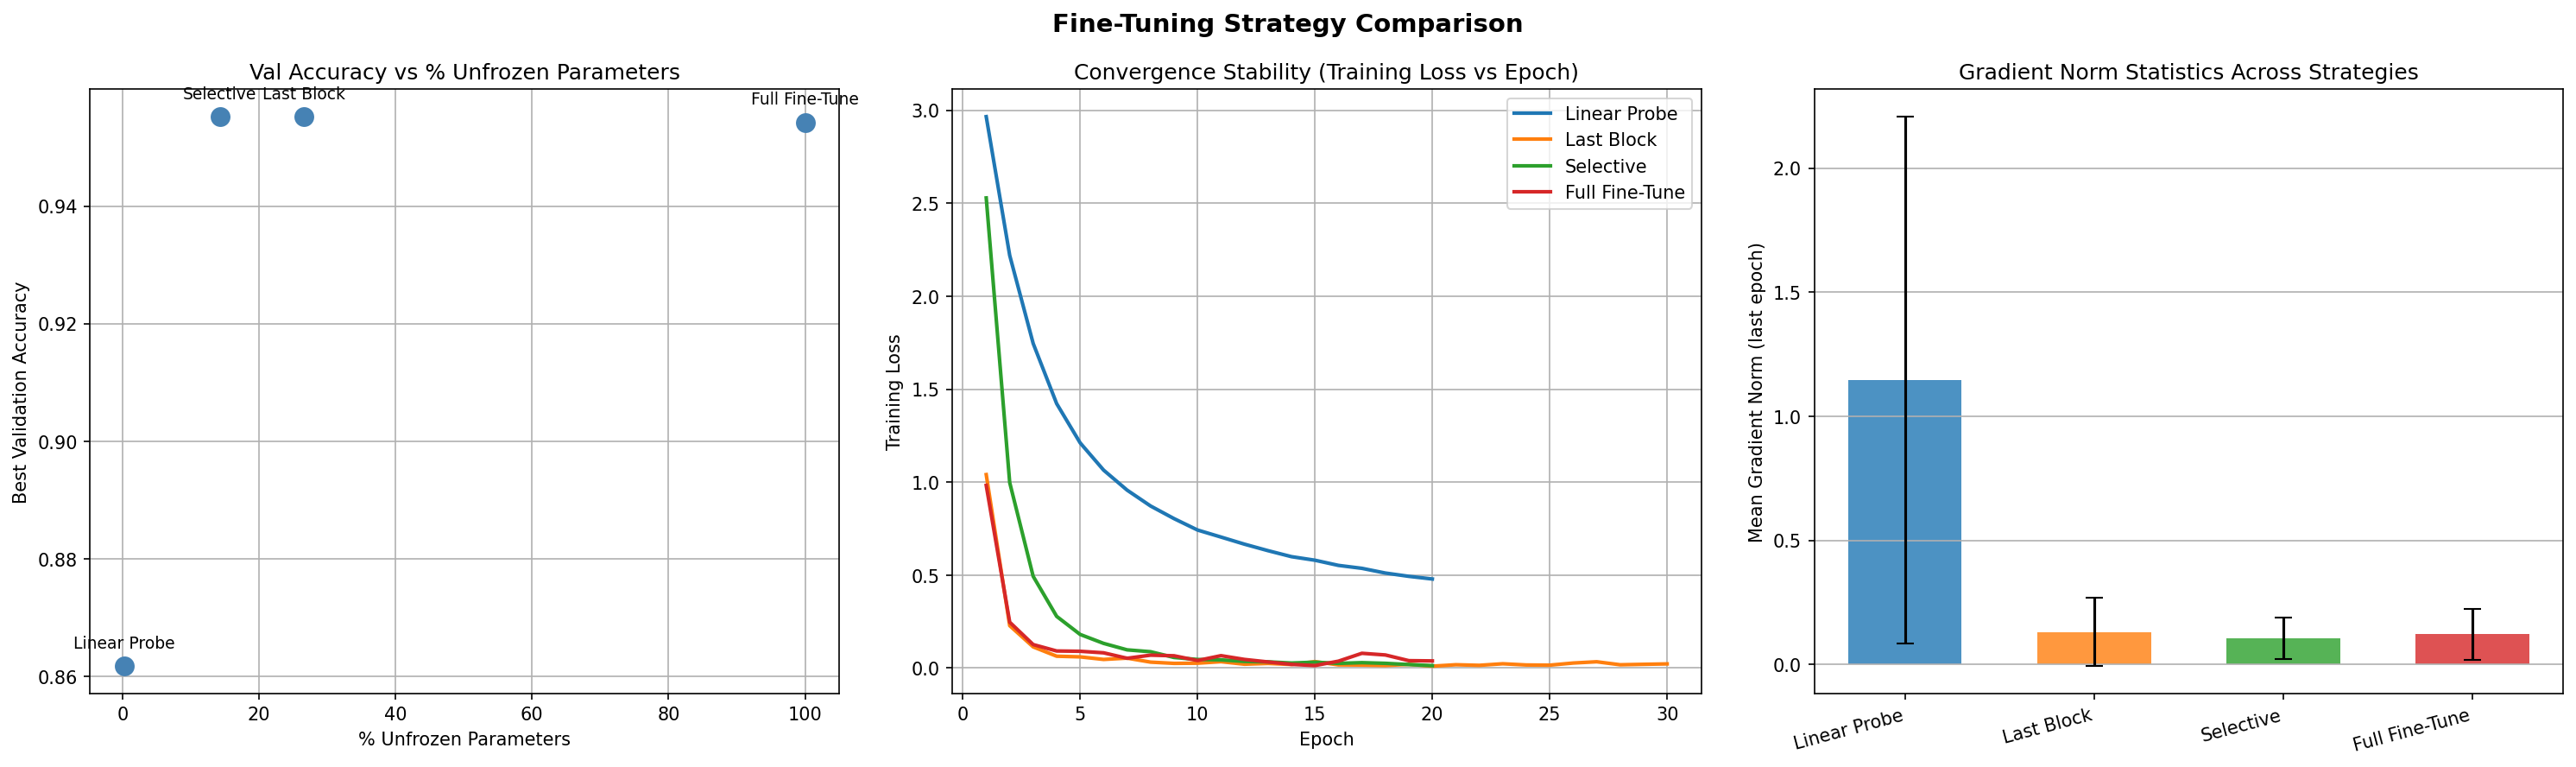
\includegraphics[width=0.9\textwidth]{../fine_tuning/resnet50_analysis.png}
	\caption{ResNet50: fine-tuning strategy comparison across linear probe, last block, selective unfreezing (14.3\%), and full fine-tuning.}
\end{figure}

\subsubsection*{EfficientNet-B0 fine-tuning comparison}
\begin{figure}[H]
	\centering
	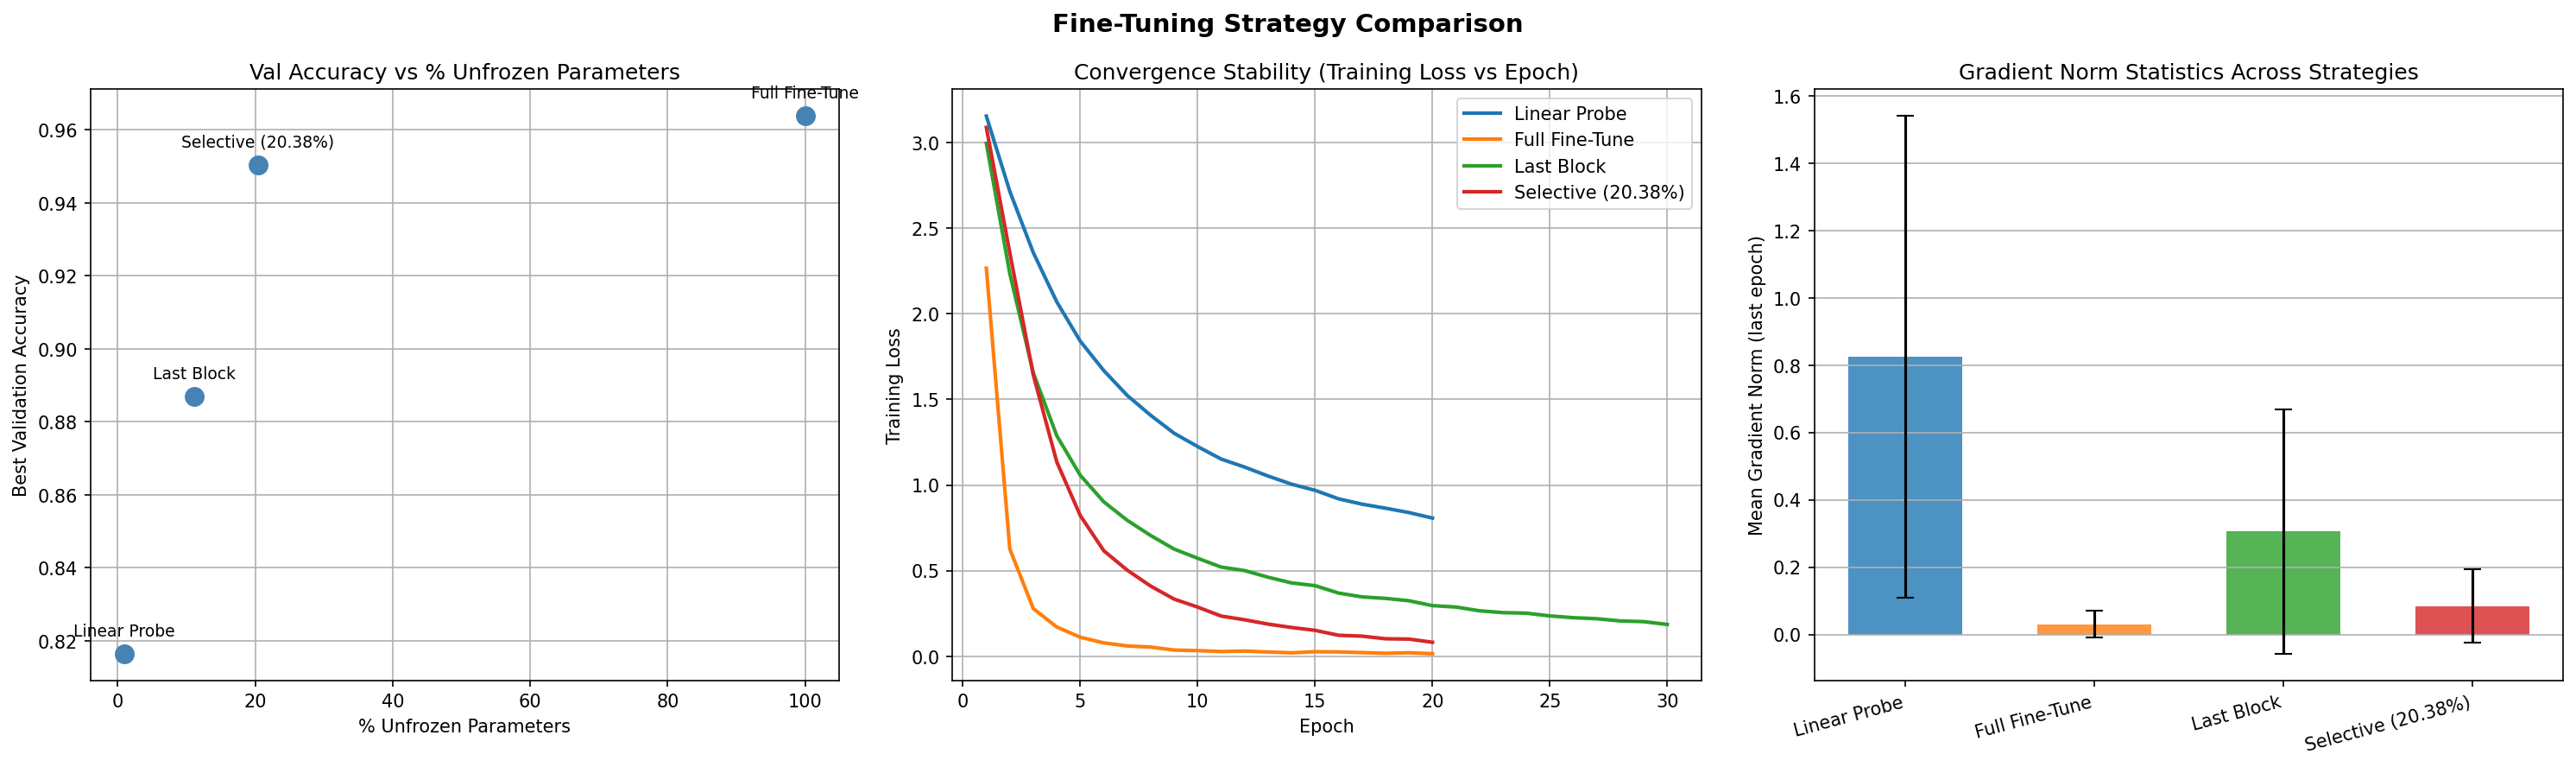
\includegraphics[width=0.9\textwidth]{../fine_tuning/efficientnet_b0_analysis.png}
	\caption{EfficientNet-B0: fine-tuning strategy comparison across linear probe, last block, selective unfreezing (20.38\%), and full fine-tuning.}
\end{figure}

\subsubsection*{ConvNeXt-Tiny fine-tuning comparison}
\begin{figure}[H]
	\centering
	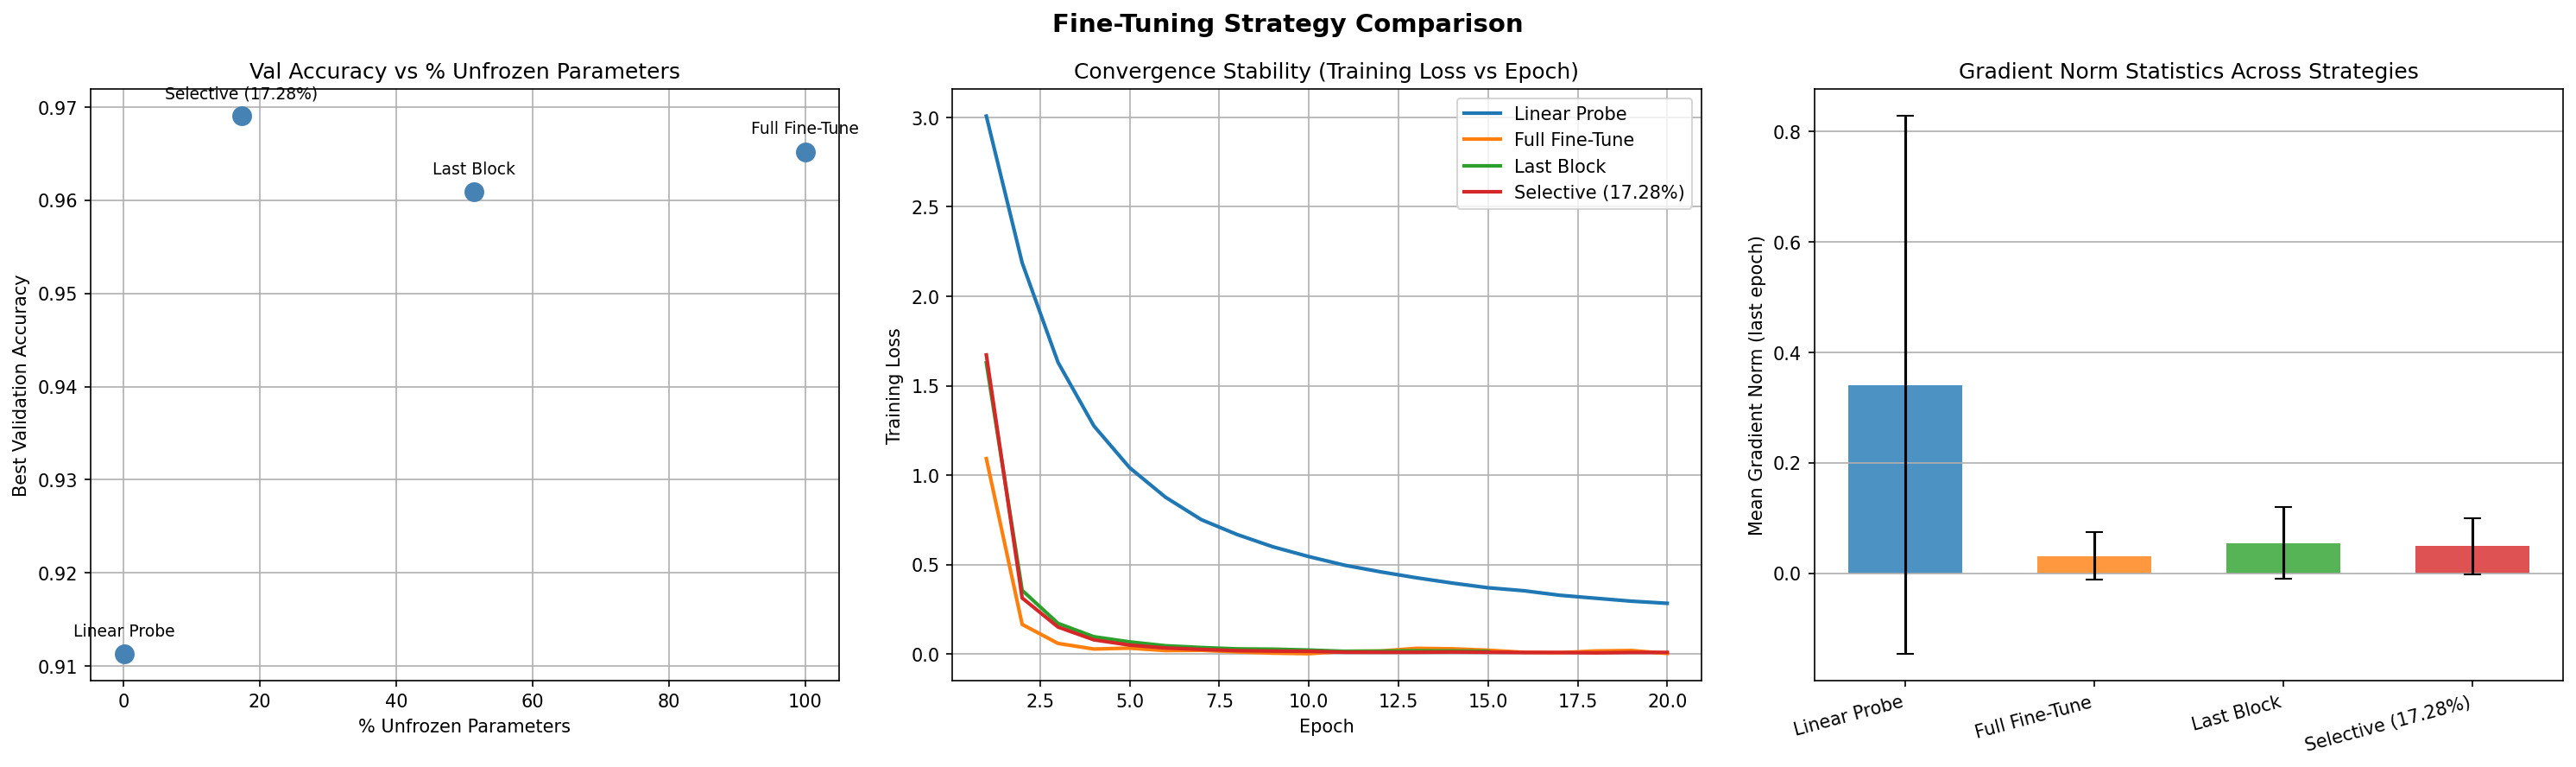
\includegraphics[width=0.9\textwidth]{../fine_tuning/convnext_tiny_analysis.png}
	\caption{ConvNeXt-Tiny: fine-tuning strategy comparison across linear probe, last block, selective unfreezing (17.28\%), and full fine-tuning.}
\end{figure}

\section{Few-Shot Learning}
\subsection{Methodology}
Few-shot performance was evaluated using the scripts in \texttt{few\_shot\_learning/} for ResNet50, EfficientNet-B0, and ConvNeXt-Tiny. For each model, we used an $80/20$ train/validation split and trained under three data regimes by subsampling the training partition: $100\%$, $20\%$, and $5\%$. All runs used seed $42$, Adam optimizer, learning rate $10^{-3}$, batch size 32, and up to 20 epochs.

For each regime, we report final validation accuracy, final training accuracy, and the training-validation gap. Following the assignment definition, relative performance drop is computed as:
\[
\Delta = \frac{\mathrm{Acc}_{100\%} - \mathrm{Acc}_{5\%}}{\mathrm{Acc}_{100\%}}.
\]

\subsection{Results}
\begin{table}[H]
	\centering
	\caption{Few-shot validation accuracy across data regimes (\%).}
	\begin{tabular}{lccc}
		\toprule
		Model & Acc@100\% & Acc@20\% & Acc@5\% \\
		\midrule
		ResNet50 & 87.20 & 66.67 & 50.29 \\
		EfficientNet-B0 & 92.49 & 90.13 & 70.03 \\
		ConvNeXt-Tiny & 89.41 & 84.69 & 61.87 \\
		\bottomrule
	\end{tabular}
\end{table}

\begin{table}[H]
	\centering
	\caption{Few-shot generalization indicators and relative drop.}
	\begin{tabular}{lccc}
		\toprule
		Model & Train-Val Gap@100\% & Train-Val Gap@5\% & $\Delta$ (100\% $\rightarrow$ 5\%) \\
		\midrule
		ResNet50 & 0.1075 & 0.4398 & 0.4233 \\
		EfficientNet-B0 & 0.0613 & 0.2782 & 0.2428 \\
		ConvNeXt-Tiny & 0.0853 & 0.3526 & 0.3080 \\
		\bottomrule
	\end{tabular}
\end{table}

\subsection{Discussion}
EfficientNet-B0 is the most data-efficient backbone in our few-shot setting. It achieves the highest validation accuracy at all three regimes and shows the smallest relative drop ($\Delta=0.2428$) from $100\%$ to $5\%$ data. ConvNeXt-Tiny is second best, while ResNet50 degrades the most under severe data scarcity ($\Delta=0.4233$).

The training-validation gap grows for all models as data reduces, indicating stronger overfitting in low-data regimes. This increase is largest for ResNet50 (0.1075 to 0.4398) and smallest for EfficientNet-B0 (0.0613 to 0.2782). Overall, these results suggest that EfficientNet-B0 transfers more robustly with limited supervision, while deeper adaptation or regularization may be necessary to stabilize ResNet50 at $5\%$ data.

These few-shot observations are consistent with the fine-tuning strategy results: constrained adaptation (e.g., selective unfreezing) is likely preferable to full fine-tuning in low-data settings where overfitting risk is high.

\section{Corruption Robustness Evaluation}
\subsection{Methodology}
Robustness was evaluated using the notebook in \texttt{corruption\_robustness\_evaluation/corruption-eval.ipynb}. Corruptions are applied only at evaluation time on normalized inputs by temporarily de-normalizing, applying the corruption in image space, clamping to $[0,1]$, and re-normalizing.

For each model (ResNet50, ConvNeXt-Tiny, EfficientNet-B0), we report clean accuracy and corrupted accuracy under:
\begin{itemize}
	\item Gaussian noise with $\sigma\in\{0.05,0.1,0.2\}$
	\item Motion blur (kernel size 15)
	\item Brightness shift (+0.2)
\end{itemize}

Metrics follow the assignment definitions:
\[
\text{Corruption Error} = 1 - \mathrm{Acc}_{\text{corrupted}}, \qquad
\text{Relative Robustness} = \frac{\mathrm{Acc}_{\text{corrupted}}}{\mathrm{Acc}_{\text{clean}}}.
\]
We additionally summarize mean corrupted accuracy across the five corruption settings.

\subsection{Results}
\begin{table}[H]
	\centering
	\caption{Corruption robustness summary across all corruption types.}
	\begin{tabular}{lcccc}
		\toprule
		Model & Clean Acc (\%) & Mean Corrupt Acc (\%) & mCE / Relative Drop & Robustness Rank \\
		\midrule
		ResNet50 & 98.34 & 59.64 & 0.4036 / 0.3936 & 2 \\
		EfficientNet-B0 & 87.12 & 25.64 & 0.7436 / 0.7057 & 3 \\
		ConvNeXt-Tiny & 96.04 & 68.36 & 0.3164 / 0.2882 & 1 \\
		\bottomrule
	\end{tabular}
\end{table}

\begin{table}[H]
	\centering
	\caption{Per-corruption accuracy (\%).}
	\begin{tabular}{lccccc}
		\toprule
		Model & Gaussian 0.05 & Gaussian 0.1 & Gaussian 0.2 & Motion Blur & Brightness \\
		\midrule
		ResNet50 & 88.72 & 45.27 & 9.97 & 57.30 & 96.93 \\
		EfficientNet-B0 & 17.76 & 1.59 & 1.64 & 23.45 & 83.74 \\
		ConvNeXt-Tiny & 88.47 & 74.36 & 39.25 & 44.50 & 95.22 \\
		\bottomrule
	\end{tabular}
\end{table}

\subsection{Discussion}
The strongest degradation comes from Gaussian noise (especially $\sigma=0.2$) and motion blur. ConvNeXt-Tiny is the most robust overall, with the highest mean corrupted accuracy (68.36\%) and the best robustness rank. ResNet50 is second: it is strong on clean and low-noise settings but drops sharply at high noise. EfficientNet-B0 is the most sensitive to corruption, with severe collapse under Gaussian noise ($\sigma\ge 0.1$).

Brightness shift is the least harmful corruption for all three models, and accuracies remain close to clean performance with relative robustness close to one. Geometric and texture distortions (blur and high noise) are therefore more challenging than global intensity changes for these pretrained backbones on the Aerial Image Dataset.

In relation to fine-tuning strategies, this suggests a useful follow-up: compare corruption robustness after selective unfreezing versus full fine-tuning to test whether the same regularization benefit also improves out-of-distribution stability.

\section{Layer-Wise Feature Probing}
\subsection{Methodology}
We probe representation quality at multiple depths by extracting intermediate activations from each frozen ImageNet-pretrained backbone and training a separate linear classifier per depth. For each selected layer output, spatial feature maps are converted to vectors through global average pooling, and a logistic-regression probe is trained on training features and evaluated on validation features.

Data handling follows the probing scripts in \texttt{layer\_wise\_feature\_probing/}: stratified $80/20$ train-validation split (seed 42), batch size 64, and fixed preprocessing from pretrained weights transforms. Layer sets are:
\begin{itemize}
	\item \textbf{ResNet50:} \texttt{early\_layer1}, \texttt{middle\_layer3}, \texttt{final\_layer4}
	\item \textbf{EfficientNet-B0:} \texttt{early\_features\_2}, \texttt{middle\_features\_4}, \texttt{final\_features\_8}
	\item \textbf{ConvNeXt-Tiny:} \texttt{early\_features\_1}, \texttt{middle\_features\_5}, \texttt{final\_features\_7}
\end{itemize}

In addition to validation accuracy versus depth, we report feature-norm statistics and PCA-2D plots on a fixed subset of 30 classes with 30 samples/class (same sampling protocol for all models/layers).

\subsection{Results and Analysis}
\begin{table}[H]
	\centering
	\caption{Layer-wise probe validation accuracy (\%).}
	\begin{tabular}{lccc}
		\toprule
		Model & Early Layer & Middle Layer & Final Layer \\
		\midrule
		ResNet50 & 85.56 & 94.92 & 91.64 \\
		EfficientNet-B0 & 66.19 & 86.85 & 92.92 \\
		ConvNeXt-Tiny & 78.34 & 95.35 & 93.57 \\
		\bottomrule
	\end{tabular}
\end{table}

\begin{table}[H]
	\centering
	\caption{Best probing depth by backbone.}
	\begin{tabular}{lcc}
		\toprule
		Model & Best Layer & Best Val Acc (\%) \\
		\midrule
		ResNet50 & middle\_layer3 & 94.92 \\
		EfficientNet-B0 & final\_features\_8 & 92.92 \\
		ConvNeXt-Tiny & middle\_features\_5 & 95.35 \\
		\bottomrule
	\end{tabular}
\end{table}

Across models, semantic separability improves strongly from early to deeper blocks. ResNet50 and ConvNeXt-Tiny peak at the middle depth, then slightly decrease at final depth, while EfficientNet-B0 improves monotonically and peaks at the final block. This indicates that optimal transfer features are architecture-dependent and not always at the deepest layer.

This layer-wise pattern also supports the fine-tuning findings: unfreezing targeted middle/deep blocks is more effective than unfreezing the full network, because the most transferable discriminative information is concentrated in specific depths.

Feature-norm statistics also show non-trivial depth behavior. For ResNet50, mean norm decreases toward final depth with higher spread in final features (std $\approx 2.75$). EfficientNet-B0 shows a high-norm middle representation before final consolidation. ConvNeXt-Tiny exhibits very low-norm early/final features with a high-norm middle layer, matching its strongest probing accuracy at middle depth.

\subsubsection*{ResNet50 probing plots}
\begin{figure}[H]
	\centering
	
\includegraphics[width=0.75\textwidth]{../layer_wise_feature_probing/resnet50_layer_wise_feature_probing/val_accuracy_vs_depth.png}
	\caption{ResNet50: validation accuracy versus probing depth.}
\end{figure}

\begin{figure}[H]
	\centering
	
\includegraphics[width=0.75\textwidth]{../layer_wise_feature_probing/resnet50_layer_wise_feature_probing/feature_norm_stats.png}
	\caption{ResNet50: feature norm statistics across selected layers.}
\end{figure}

\begin{figure}[H]
	\centering
	
\includegraphics[width=0.75\textwidth]{../layer_wise_feature_probing/resnet50_layer_wise_feature_probing/pca_2d_across_layers.png}
	\caption{ResNet50: PCA-2D projection across early/middle/final layers.}
\end{figure}

\subsubsection*{EfficientNet-B0 probing plots}
\begin{figure}[H]
	\centering
	
\includegraphics[width=0.75\textwidth]{../layer_wise_feature_probing/efficientnet_bo_layer_wise_feature_probing/val_accuracy_vs_depth.png}
	\caption{EfficientNet-B0: validation accuracy versus probing depth.}
\end{figure}

\begin{figure}[H]
	\centering
	
\includegraphics[width=0.75\textwidth]{../layer_wise_feature_probing/efficientnet_bo_layer_wise_feature_probing/feature_norm_stats.png}
	\caption{EfficientNet-B0: feature norm statistics across selected layers.}
\end{figure}

\begin{figure}[H]
	\centering
	
\includegraphics[width=0.75\textwidth]{../layer_wise_feature_probing/efficientnet_bo_layer_wise_feature_probing/pca_2d_across_layers.png}
	\caption{EfficientNet-B0: PCA-2D projection across early/middle/final layers.}
\end{figure}

\subsubsection*{ConvNeXt-Tiny probing plots}
\begin{figure}[H]
	\centering
	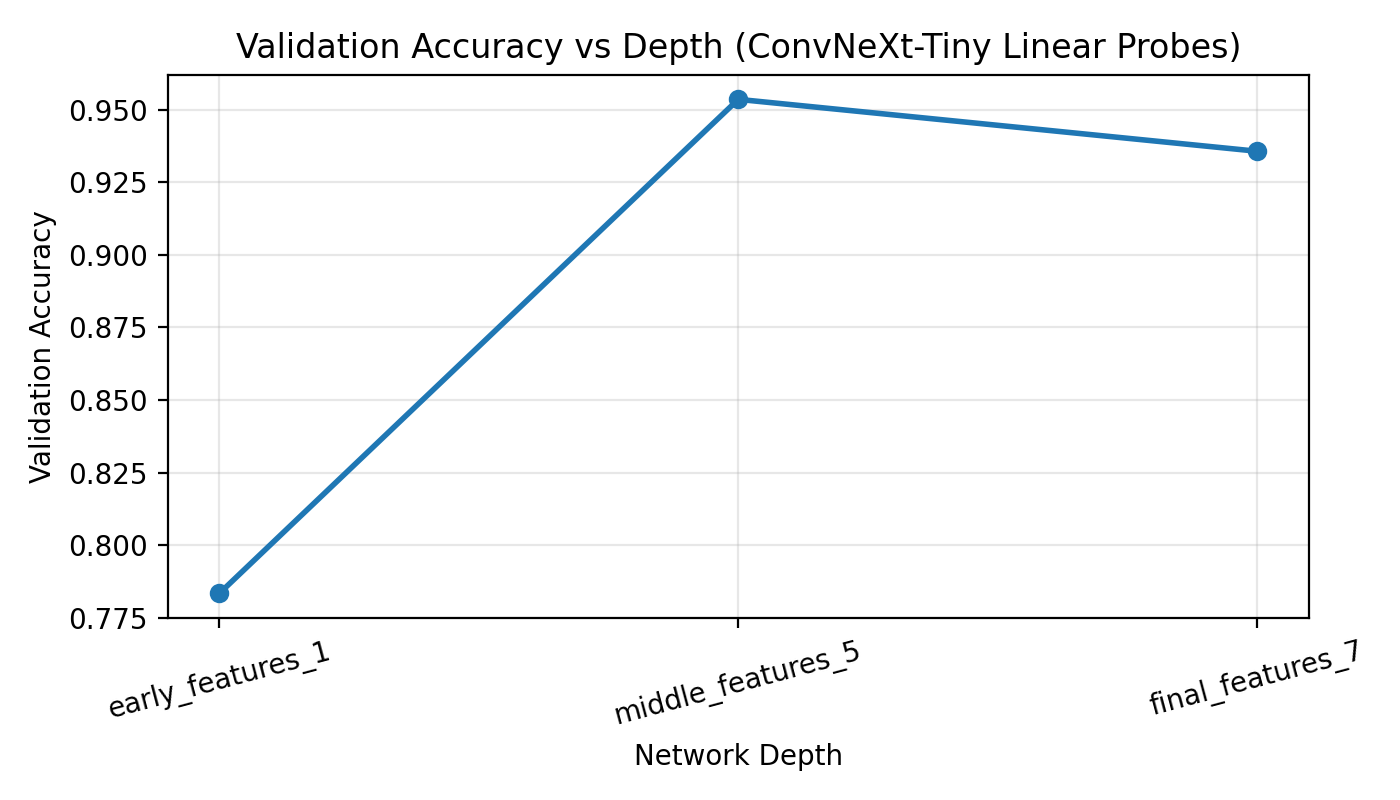
\includegraphics[width=0.75\textwidth]{../layer_wise_feature_probing/convnext_tiny_layer_wise_feature_probing/val_accuracy_vs_depth.png}
	\caption{ConvNeXt-Tiny: validation accuracy versus probing depth.}
\end{figure}

\begin{figure}[H]
	\centering
	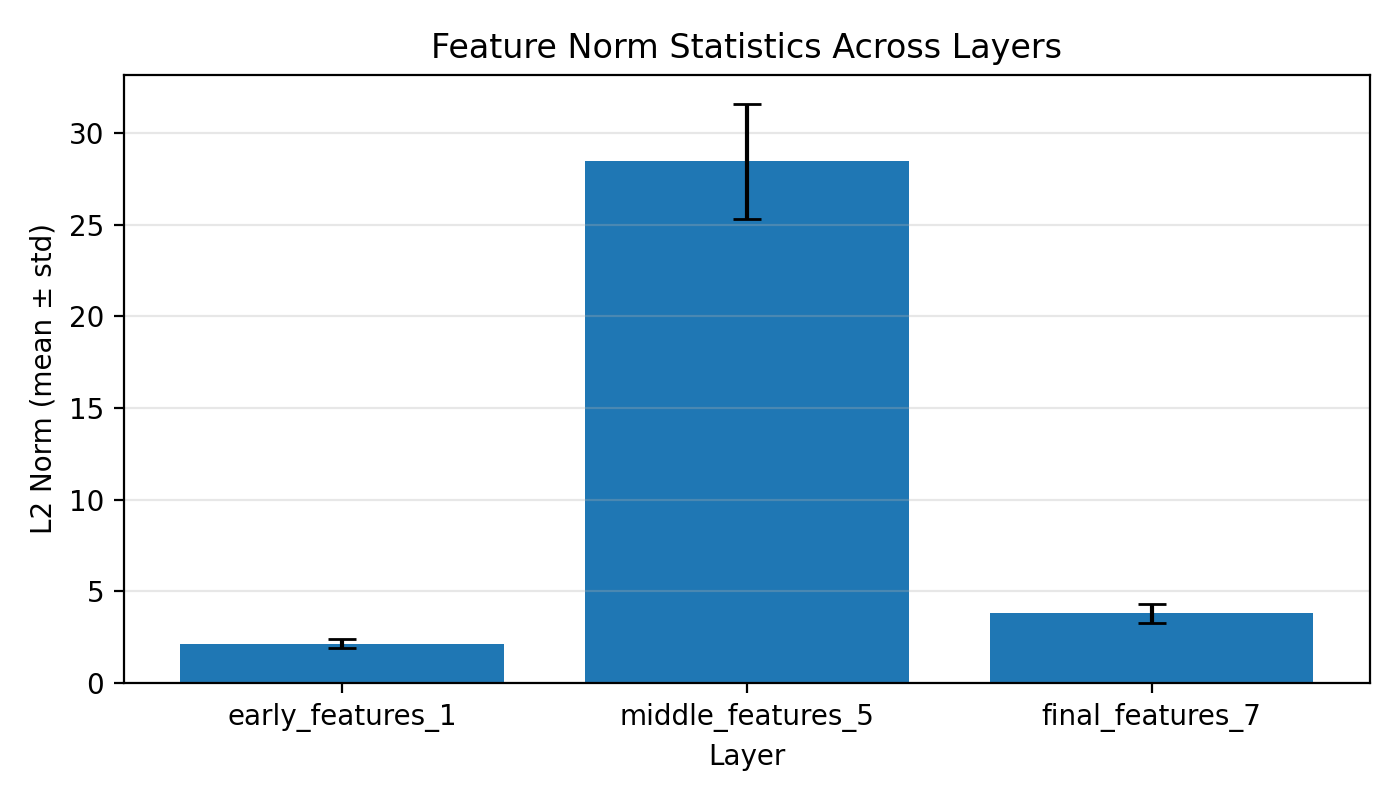
\includegraphics[width=0.75\textwidth]{../layer_wise_feature_probing/convnext_tiny_layer_wise_feature_probing/feature_norm_stats.png}
	\caption{ConvNeXt-Tiny: feature norm statistics across selected layers.}
\end{figure}

\begin{figure}[H]
	\centering
	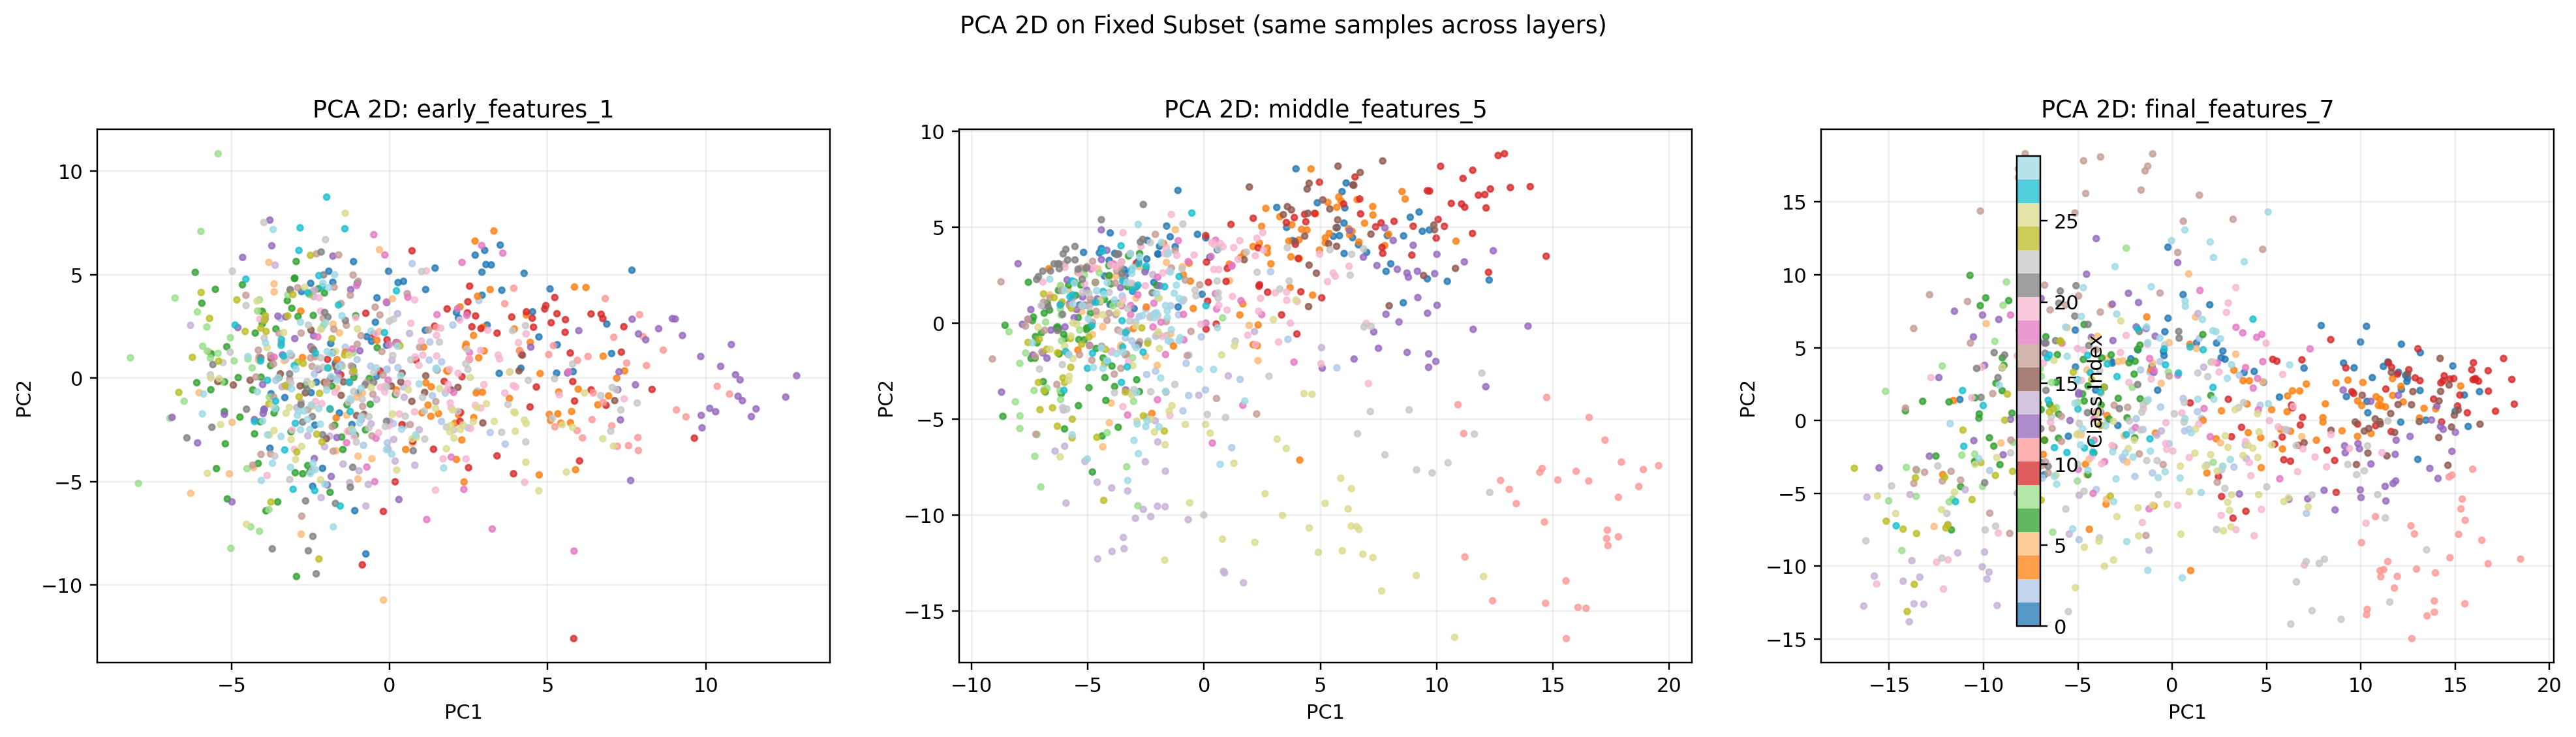
\includegraphics[width=0.75\textwidth]{../layer_wise_feature_probing/convnext_tiny_layer_wise_feature_probing/pca_2d_across_layers.png}
	\caption{ConvNeXt-Tiny: PCA-2D projection across early/middle/final layers.}
\end{figure}

\section{Consolidated Comparison}
\begin{table}[H]
	\centering
	\caption{Unified comparison across reported tasks (three selected backbones).}
	\resizebox{\textwidth}{!}{%
	\begin{tabular}{lccccc}
		\toprule
		Model & Few-shot Acc@5\% & Best Probe Acc & Transfer Val Acc & Best FT Val Acc (strategy) & Mean Corrupt Acc \\
		\midrule
		ResNet50 & 50.29 & 94.92 & 98.28 & 95.52 (last/selective) & 59.64 \\
		EfficientNet-B0 & 70.03 & 92.92 & 87.37 & 96.38 (full FT) & 25.64 \\
		ConvNeXt-Tiny & 61.87 & 95.35 & 95.28 & 96.90 (selective) & 68.36 \\
		\bottomrule
	\end{tabular}%
	}
\end{table}

Overall ranking by task is not identical: EfficientNet-B0 leads few-shot data efficiency, ConvNeXt-Tiny leads probing depth quality and robustness, and ResNet50 shows excellent logged linear-probe transfer. This supports the central conclusion that no single backbone dominates all criteria under the same dataset and protocol.

From the fine-tuning comparison, a practical insight is that the optimal adaptation budget is architecture-dependent: constrained unfreezing is competitive or best for ResNet50/ConvNeXt-Tiny, while EfficientNet-B0 benefits most from full fine-tuning in this run.

\section{Conclusion and Future Work}
Key conclusions from this study are:
\begin{itemize}
	\item \textbf{Few-shot:} EfficientNet-B0 is most data-efficient, with the highest $5\%$-data validation accuracy and smallest relative drop.
	\item \textbf{Fine-tuning strategies:} The best strategy is model-dependent: ResNet50 performs best with last-block/selective unfreezing (tie at 95.52\%), EfficientNet-B0 peaks with full fine-tuning (96.38\%), and ConvNeXt-Tiny peaks with selective unfreezing (96.90\%).
	\item \textbf{Layer-wise probing:} Mid-to-late representations are substantially more separable than early features; ConvNeXt-Tiny attains the best peak probe accuracy.
	\item \textbf{Linear transfer:} Frozen-pretrained features are highly transferable on AID, with ResNet50 reaching very high logged validation performance.
	\item \textbf{Robustness:} ConvNeXt-Tiny is most robust to corruption overall, while EfficientNet-B0 is highly sensitive to Gaussian noise.
	\item \textbf{Cross-task insight:} Backbone and adaptation strategy should be objective-driven (data efficiency vs robustness vs transfer vs parameter budget), rather than based on a single metric.
\end{itemize}

Main limitations of the current study are:
\begin{itemize}
	\item Corruption robustness was evaluated at model level, but not recomputed for each fine-tuning strategy (linear probe, last-block, selective, full); therefore strategy-level robustness conclusions remain indirect.
	\item Protocols differ across sections (e.g., $70/30$ for transfer/fine-tuning vs $80/20$ for few-shot/probing), which is suitable for assignment tasks but limits strict cross-section comparability.
	\item Robustness coverage is limited to three corruption families (Gaussian noise, motion blur, brightness), and does not include additional real-world shifts such as compression artifacts, haze, scale/viewpoint variation, or seasonal changes.
	\item Results are from single-seed runs per setting in the current report; uncertainty estimates (mean$\pm$std across multiple seeds) are not reported.
\end{itemize}

Future work directions include:
\begin{itemize}
	\item Re-run corruption evaluation for every fine-tuning strategy and report strategy-specific robustness metrics (mCE, relative robustness, and calibration under shift).
	\item Standardize train/validation protocols across sections and add multi-seed evaluation to improve fairness and statistical confidence.
	\item Expand distribution-shift benchmarks to additional corruptions and domain shifts relevant to aerial imagery (weather, compression, resolution, viewpoint, and temporal shift).
	\item Investigate robustness-oriented adaptation methods (corruption augmentation, SAM/weight averaging, adversarial-style training, and domain adaptation) and compare their trade-offs against clean accuracy.
\end{itemize}

\begin{thebibliography}{9}
\bibitem{he2016resnet}
K. He, X. Zhang, S. Ren, and J. Sun, Deep Residual Learning for Image Recognition, CVPR, 2016.

\bibitem{tan2019efficientnet}
M. Tan and Q. Le, EfficientNet: Rethinking Model Scaling for Convolutional Neural Networks, ICML, 2019.

\bibitem{liu2022convnext}
Z. Liu \textit{et al.}, A ConvNet for the 2020s, CVPR, 2022.
\end{thebibliography}

\end{document}
